\documentclass[12pt,a4paper]{article}

% ─── Packages ────────────────────────────────────────────────────────────────
\usepackage[utf8]{inputenc}
\usepackage[T1]{fontenc}
\usepackage[english]{babel}
\usepackage{geometry}
\geometry{margin=2.5cm}

\usepackage{amsmath,amssymb,amsthm}
\usepackage{graphicx}
\usepackage{float}
\usepackage{booktabs}
\usepackage{longtable}
\usepackage{multirow}
\usepackage{array}
\usepackage{xcolor}
\usepackage{hyperref}
\usepackage{listings}
\usepackage{caption}
\usepackage{subcaption}
\usepackage{enumitem}
\usepackage{fancyhdr}
\usepackage{titlesec}
\usepackage{abstract}
\usepackage{setspace}
\usepackage{microtype}

% TikZ
\usepackage{tikz}
\usetikzlibrary{shapes.geometric, arrows.meta, positioning, fit, backgrounds,
                decorations.pathreplacing, calc, patterns, shadows}

% Code listings style
\definecolor{codebg}{RGB}{248,248,252}
\definecolor{codeframe}{RGB}{200,200,215}
\definecolor{keyword}{RGB}{0,112,192}
\definecolor{string}{RGB}{163,21,21}
\definecolor{comment}{RGB}{100,130,90}

\lstdefinestyle{tscode}{
  backgroundcolor=\color{codebg},
  frame=single,
  rulecolor=\color{codeframe},
  basicstyle=\ttfamily\small,
  keywordstyle=\color{keyword}\bfseries,
  stringstyle=\color{string},
  commentstyle=\color{comment}\itshape,
  breaklines=true,
  showstringspaces=false,
  tabsize=2,
  numbers=left,
  numberstyle=\tiny\color{gray},
  numbersep=8pt,
}

% Custom colors
\definecolor{israelblue}{RGB}{0,56,184}
\definecolor{israelwhite}{RGB}{255,255,255}
\definecolor{azureblue}{RGB}{56,189,248}
\definecolor{emerald}{RGB}{16,185,129}
\definecolor{sectioncolor}{RGB}{0,56,184}

% Section formatting
\titleformat{\section}{\large\bfseries\color{sectioncolor}}{{\thesection}}{1em}{}[\titlerule]
\titleformat{\subsection}{\normalsize\bfseries\color{sectioncolor}}{{\thesubsection}}{1em}{}
\titleformat{\subsubsection}{\normalsize\bfseries}{{\thesubsubsection}}{1em}{}

% Header/Footer
\pagestyle{fancy}
\fancyhf{}
\fancyhead[L]{\small\textit{Israel Shield — Security Intelligence Dashboard}}
\fancyhead[R]{\small\textit{Ariel University, 2026}}
\fancyfoot[C]{\thepage}
\renewcommand{\headrulewidth}{0.4pt}

% Hyperref
\hypersetup{
  colorlinks=true,
  linkcolor=israelblue,
  citecolor=israelblue,
  urlcolor=azureblue,
  pdftitle={Israel Shield: A Real-Time Security Intelligence Dashboard},
  pdfauthor={Ariel University BI Course},
}

% Theorem environments
\newtheorem{definition}{Definition}
\newtheorem{proposition}{Proposition}

% ─── Document ─────────────────────────────────────────────────────────────────
\begin{document}

\begin{titlepage}
  \centering
  \vspace*{1cm}

  % Shield TikZ logo
  
\begin{tikzpicture}
    \begin{scope}[transform canvas={scale=1.2}]
      % Shield shape
      \fill[israelblue!90] (0,0) -- (2.2,0) -- (2.2,2.5) arc (0:180:1.1) -- cycle;
      \fill[white,opacity=0.15] (0.3,0.3) -- (1.9,0.3) -- (1.9,2.3) arc(0:180:0.8) -- cycle;
      % Star of David
      \draw[white,line width=2pt] (1.1,1.1) -- ++(60:0.7) -- ++(180:0.7) -- cycle;
      \draw[white,line width=2pt] (1.1,1.8) -- ++(-60:0.7) -- ++(60:0.7) -- cycle;
    \end{scope}
  \end{tikzpicture}

  \vspace{0.8cm}
  {\Huge\bfseries\color{israelblue} Israel Shield}\\[0.4cm]
  {\Large\bfseries A Real-Time Security Intelligence Dashboard}\\[0.3cm]
  {\large for Threat Pattern Analysis and Safe Navigation}

  \vspace{1.2cm}
  \rule{0.7\linewidth}{0.4pt}\\[0.3cm]

  \begin{tabular}{rl}
    \textbf{Institution:} & Ariel University, Department of Industrial Engineering \\
    \textbf{Course:}       & Business Intelligence \\
    \textbf{Supervisor:}   & Dr. Guy Wachtel \\
    \textbf{Data Source:}  & IDF Home Front Command \& Dr. Yuval Harpaz \\
    \textbf{Year:}         & 2025--2026 \\
  \end{tabular}

  \vspace{1.2cm}
  \rule{0.7\linewidth}{0.4pt}

  \vspace{0.8cm}
  \textit{Dedicated to the memory of the victims of October 7th, 2023,\\
  and all those who have fallen in the ongoing conflict.}

  \vfill
  \today
\end{titlepage}

% ─── Abstract ──────────────────────────────────────────────────────────────
\begin{abstract}
\noindent
We present \textbf{Israel Shield}, a browser-based, real-time security intelligence dashboard that aggregates, analyzes, and visualizes over a decade of rocket, missile, drone, and terrorist infiltration alerts across Israel. The system integrates a live alert feed from the IDF Home Front Command with a curated historical dataset of 10,000+ records spanning 2019--2026, processing them through a suite of statistical and algorithmic models. Key contributions include: (1) a \emph{Spatio-Temporal UAV Route Reconstruction} algorithm that chains historical drone alert sequences into probable flight trajectories; (2) a \emph{Safe Route Departure Advisor} that scores every departure hour using a sliding window aggregation over historical threat corridors along a travel path; (3) a \emph{Shower Index} probabilistic safety estimator based on Poisson statistics; and (4) a fully client-side, offline-capable progressive web application supporting seven languages and bidirectional text. The system demonstrates that meaningful security analytics are achievable without proprietary infrastructure, enabling both civilian and academic use cases.

\medskip
\noindent\textbf{Keywords:} security analytics, threat visualization, spatio-temporal analysis, UAV tracking, safe route planning, business intelligence, homeland security, Israel.
\end{abstract}

\tableofcontents
\newpage

% ─────────────────────────────────────────────────────────────────────────────
\section{Introduction}
\label{sec:introduction}
% ─────────────────────────────────────────────────────────────────────────────

Since 2001, Israel has faced continuous rocket fire, and since 2023, an unprecedented escalation of multi-front hostilities involving rockets, ballistic missiles, cruise missiles, and unmanned aerial vehicles (UAVs) from Gaza, Lebanon, Iran, Yemen, Iraq, and Syria simultaneously. The IDF Home Front Command (\textit{Pikud HaOref}) operates a public alert system that has generated a historically unique dataset: a timestamped, city-level record of every incoming threat warning issued to the Israeli civilian population.

This dataset presents an extraordinary opportunity for \emph{threat pattern analysis} — the systematic study of \emph{when}, \emph{where}, and \emph{how} security incidents occur at a population level. Despite its public availability, no accessible, multi-functional analytical tool existed that combined this data with real-time feeds, geographic visualization, probabilistic safety estimation, and navigation planning.

\textbf{Israel Shield} fills this gap. It is a full-stack web application, built as a Business Intelligence project at Ariel University, that transforms the raw alert record into actionable intelligence for civilians, researchers, and policy analysts. Its key distinguishing features are:

\begin{enumerate}
  \item \textbf{UAV Route Reconstruction}: A novel spatio-temporal chaining algorithm that reconstructs probable drone flight trajectories from the time-ordered sequence of city alert activations.
  \item \textbf{Safe Route Planner}: A departure time optimization system that scores each hour of day based on historical threat intensity along a proposed travel corridor.
  \item \textbf{Shower Index}: A Poisson-based daily safety window estimator — colloquially named for the quintessential civilian dilemma of "is it safe to shower right now?"
  \item \textbf{Multi-dimensional temporal analysis} across seven temporal resolutions (year, month, weekday, hour, minute, daytime, date).
  \item \textbf{Full offline capability} via IndexedDB caching and Progressive Web App (PWA) support.
\end{enumerate}

The remainder of this paper is organized as follows. Section~\ref{sec:background} reviews related work. Section~\ref{sec:data} describes the data sources and processing pipeline. Section~\ref{sec:architecture} details the system architecture. Sections~\ref{sec:uav}--\ref{sec:shower} describe the statistical and algorithmic models. Section~\ref{sec:ui} describes the user interface. Section~\ref{sec:implementation} discusses implementation choices and performance. Section~\ref{sec:evaluation} evaluates the system. Section~\ref{sec:future} outlines future directions, and Section~\ref{sec:conclusion} concludes.

% ─────────────────────────────────────────────────────────────────────────────
\section{Background and Related Work}
\label{sec:background}
% ─────────────────────────────────────────────────────────────────────────────

\subsection{Open Security Data in Israel}

The Israeli Home Front Command's alert system (\textit{Red Alert / Tzeva Adom}) is one of the world's most densely documented civilian warning datasets. Since 2001, alerts have been issued at the city level, timestamped to the second, and made publicly accessible via a JSON API. Academic use of this data has been limited; most analyses have been journalistic or statistical in nature \cite{harpaz2023}.

\subsection{Threat Visualization Systems}

Existing threat visualization platforms (e.g., LiveUA Map, ACLED) focus on macro-level geographic conflict mapping without city-level temporal granularity. None incorporate the IDF alert feed's precision.

\subsection{UAV Trajectory Reconstruction}

UAV trajectory inference from indirect observations is an active research area in air traffic management \cite{olive2019}. Prior work typically requires ADS-B transponder data or radar returns. This paper presents the first method applied to civilian warning activations as a proxy for trajectory reconstruction.

\subsection{Route Safety Planning}

Route safety planning in conflict zones has been studied in humanitarian logistics \cite{tomasini2009}. Most approaches use road network graph algorithms (Dijkstra, A*) with risk weights per edge. Our approach differs: we compute temporal rather than spatial risk, optimizing \emph{when} to travel rather than \emph{which road} to take.

\subsection{Poisson Models for Safety Windows}

Poisson processes are standard models for rare event occurrence in time \cite{kingman1992}. The Shower Index applies Poisson statistics to compute the probability of a zero-alert interval within a 30-minute window.

% ─────────────────────────────────────────────────────────────────────────────
\section{Data Sources and Processing Pipeline}
\label{sec:data}
% ─────────────────────────────────────────────────────────────────────────────

\subsection{Data Sources}

\subsubsection{Historical Alert Dataset}

The primary data source is a community-curated CSV maintained by Dr. Yuval Harpaz on GitHub (\texttt{yuval-harpaz/alarms}). Each record contains:

\begin{table}[H]
\centering
\caption{Alert Record Schema}
\begin{tabular}{lll}
\toprule
\textbf{Field} & \textbf{Type} & \textbf{Description} \\
\midrule
\texttt{time}     & String  & ISO timestamp (e.g., \texttt{2023-10-07 06:29:00}) \\
\texttt{cities}   & String  & Hebrew city/region name \\
\texttt{threat}   & String  & Numeric code or Hebrew threat category \\
\texttt{category} & String  & Alternative threat field (some records) \\
\texttt{id}       & String  & Optional event ID (IDF batch identifier) \\
\bottomrule
\end{tabular}
\end{table}

\noindent The dataset contains $N \approx 10{,}000+$ records spanning 2019--2026, with density increasing dramatically from October 2023.

\subsubsection{Live Alert Feed}

Real-time alerts are fetched via:
\begin{center}
\texttt{https://www.oref.org.il/WarningMessages/alert/alerts.json}
\end{center}
due to CORS restrictions, accessed via the \texttt{allorigins.win} proxy. Polling is performed every 10 seconds.

\subsubsection{Geographic Coordinates}

A \texttt{baseCoords} dictionary hardcodes coordinates for 450+ Israeli cities, settlements, and regions. This covers the Gaza Envelope (Otef Aza), the northern border (Upper Galilee, Golan Heights), central Israel, the Negev, and all major population centers. For cities not in \texttt{baseCoords}, the OpenStreetMap Nominatim API is queried dynamically with rate limiting (1 request/second, 20 cities/batch), and results are cached in \texttt{localStorage}.

\subsection{Data Processing Pipeline}

Figure~\ref{fig:pipeline} shows the end-to-end data pipeline.

\begin{figure}[H]
\centering
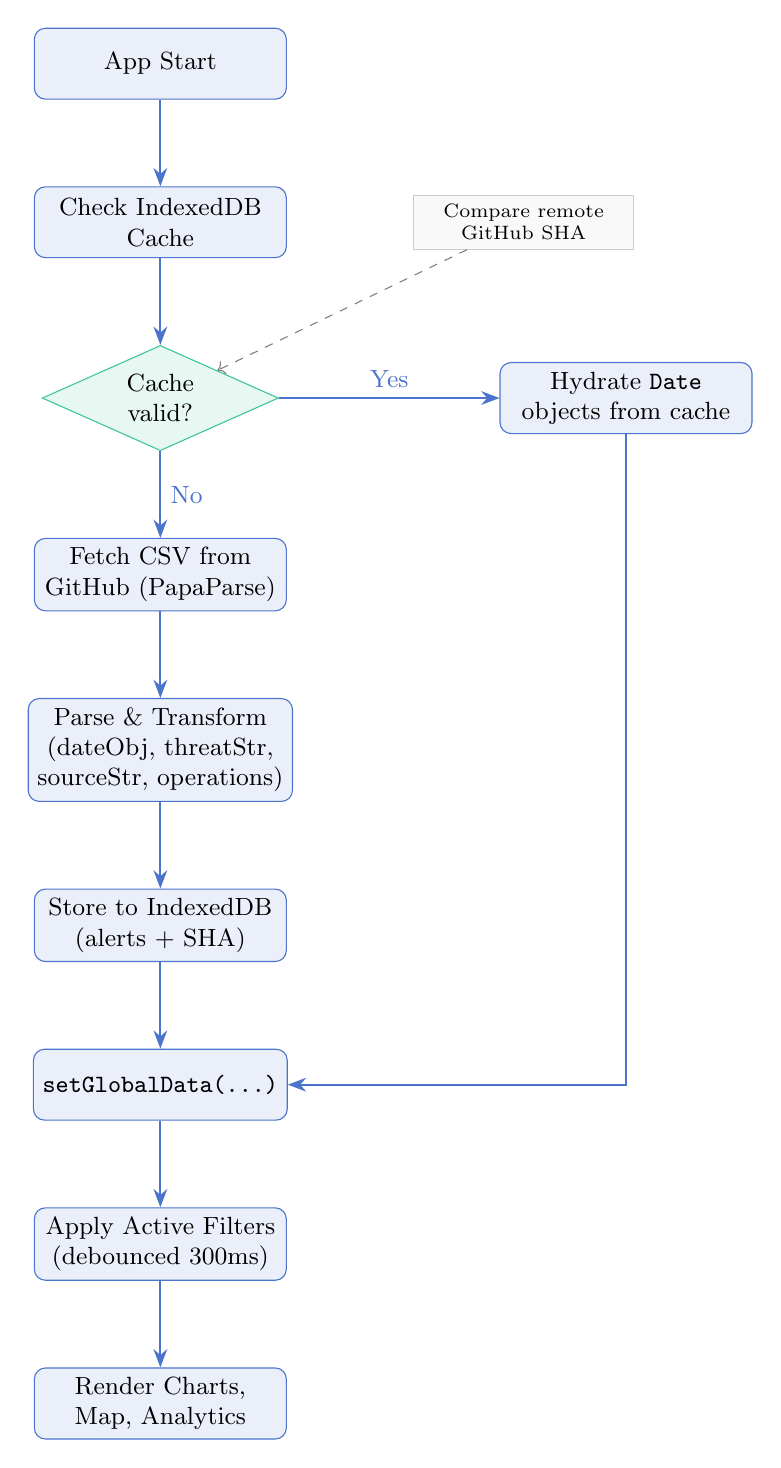
\begin{tikzpicture}[
  node distance=1.1cm and 2.2cm,
  box/.style={rectangle, rounded corners=4pt, draw=israelblue!70, fill=israelblue!8,
              minimum width=3.2cm, minimum height=0.9cm, align=center, font=\small},
  decision/.style={diamond, draw=emerald!80, fill=emerald!10, aspect=2.2,
                   minimum width=3cm, align=center, font=\small},
  arrow/.style={-Stealth, thick, color=israelblue!70},
  note/.style={rectangle, draw=gray!40, fill=gray!5, font=\scriptsize,
               minimum width=2.8cm, align=center},
]
  \node[box] (start)   {App Start};
  \node[box, below=of start] (cache) {Check IndexedDB\\Cache};
  \node[decision, below=of cache] (valid) {Cache\\valid?};
  \node[box, right=2.8cm of valid] (hydrate) {Hydrate \texttt{Date}\\objects from cache};
  \node[box, below=of valid] (fetch)  {Fetch CSV from\\GitHub (PapaParse)};
  \node[box, below=of fetch]  (parse)  {Parse \& Transform\\(dateObj, threatStr,\\sourceStr, operations)};
  \node[box, below=of parse]  (store)  {Store to IndexedDB\\(alerts + SHA)};
  \node[box, below=of store, minimum width=3.2cm] (state)  {\texttt{setGlobalData(\ldots)}};
  \node[box, below=of state]  (filter) {Apply Active Filters\\(debounced 300ms)};
  \node[box, below=of filter] (render) {Render Charts,\\Map, Analytics};

  \draw[arrow] (start)  -- (cache);
  \draw[arrow] (cache)  -- (valid);
  \draw[arrow] (valid)  -- node[right,font=\small]{No} (fetch);
  \draw[arrow] (valid)  -- node[above,font=\small]{Yes} (hydrate);
  \draw[arrow] (hydrate) |- (state);
  \draw[arrow] (fetch)  -- (parse);
  \draw[arrow] (parse)  -- (store);
  \draw[arrow] (store)  -- (state);
  \draw[arrow] (state)  -- (filter);
  \draw[arrow] (filter) -- (render);

  % SHA note
  \node[note, right=1.6cm of cache] (sha) {Compare remote\\GitHub SHA};
  \draw[->, dashed, gray] (sha) -- (valid);
\end{tikzpicture}
\caption{Data loading and processing pipeline.}
\label{fig:pipeline}
\end{figure}

\subsubsection{Threat Classification}

Threat types are extracted from numeric codes and keyword patterns in the raw data:

\begin{table}[H]
\centering
\caption{Threat Type Taxonomy}
\begin{tabular}{lll}
\toprule
\textbf{Code/Pattern} & \textbf{Hebrew} & \textbf{English} \\
\midrule
1 / ירי   & ירי רקטות וטילים & Rocket \& Missile Fire \\
2 / כטב"מ & חדירת כלי טיס עוין & Hostile Aircraft Intrusion \\
3         & רעידת אדמה         & Earthquake \\
4         & אירוע רדיולוגי     & Radiological Incident \\
5 / מחבלים & חדירת מחבלים      & Terrorist Infiltration \\
6         & צונאמי             & Tsunami \\
7         & חומרים מסוכנים     & Hazardous Materials \\
8         & אירוע לא קונבנציונלי & Non-Conventional Event \\
--        & אחר               & Other \\
\bottomrule
\end{tabular}
\end{table}

\subsubsection{Source Attribution}

Threat sources are inferred via keyword matching in raw data fields plus geographic heuristics:
\begin{itemize}
  \item Raw field contains "איראן" $\Rightarrow$ Iran
  \item Alert city is in the Gaza Envelope $\Rightarrow$ Gaza Strip (default for rockets)
  \item Alert city is on northern border (e.g., Kiryat Shmona) $\Rightarrow$ Lebanon
  \item Operation date overlaps with known Iranian strikes $\Rightarrow$ Iran
\end{itemize}

\subsubsection{Operation Assignment}

Each alert is assigned to one or more named military operations based on its timestamp. The operations dictionary defines 10 operations:

\begin{table}[H]
\centering
\caption{Named Military Operations in the Dataset}
\begin{tabular}{lll}
\toprule
\textbf{Name (Hebrew)} & \textbf{Dates} & \textbf{Theater} \\
\midrule
חגורה שחורה (2019) & Nov 12--14, 2019 & Gaza \\
שומר החומות (2021) & May 10--21, 2021 & Gaza, Lebanon \\
עלות השחר (2022) & Aug 5--7, 2022 & Gaza \\
מגן וחץ (2023) & May 9--13, 2023 & Gaza \\
חרבות ברזל (2023+) & Oct 7, 2023 -- present & Multi-front \\
מתקפת אפריל — איראן (2024) & Apr 13--14, 2024 & Iran \\
מתקפת אוקטובר — איראן (2024) & Oct 1, 2024 & Iran \\
ימי תשובה — איראן (2024) & Oct 26--27, 2024 & Iran \\
עם כלביא — איראן (2025) & Jun 13--24, 2025 & Iran \\
כארי ישאג — איראן (2026) & Feb 28 -- Mar 31, 2026 & Iran \\
\bottomrule
\end{tabular}
\end{table}

% ─────────────────────────────────────────────────────────────────────────────
\section{System Architecture}
\label{sec:architecture}
% ─────────────────────────────────────────────────────────────────────────────

\subsection{Technology Stack}

\begin{table}[H]
\centering
\caption{Technology Stack}
\begin{tabular}{ll}
\toprule
\textbf{Layer} & \textbf{Technology} \\
\midrule
Frontend framework & React 19 + TypeScript \\
Build tool & Vite 6.2 \\
Styling & Tailwind CSS 4.1 + CSS custom properties \\
Charts & Apache ECharts 6 via \texttt{echarts-for-react} \\
Mapping & Leaflet 1.9 (CartoDB Light + ESRI Satellite tiles) \\
Animations & Framer Motion \\
CSV parsing & PapaParse 5.5 (web worker) \\
Data caching & Browser IndexedDB \\
Geocoding & OpenStreetMap Nominatim \\
Road routing & OSRM public API \\
Live alerts & \texttt{oref.org.il} via CORS proxy \\
Analytics & Vercel Analytics 2.0 \\
AI (planned) & Google GenAI SDK 1.29 \\
\bottomrule
\end{tabular}
\end{table}

\subsection{Component Architecture}

Figure~\ref{fig:components} shows the high-level component hierarchy.

\begin{figure}[H]
\centering
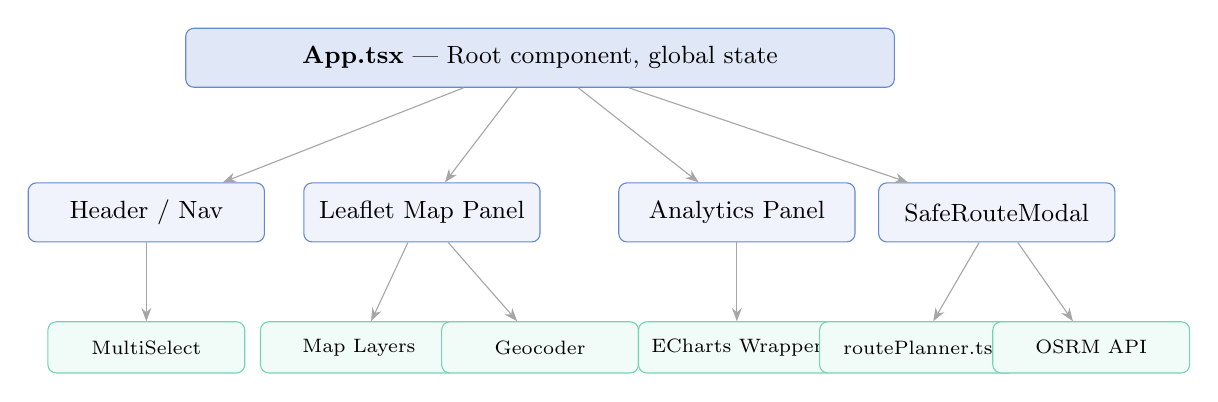
\begin{tikzpicture}[
  comp/.style={rectangle, rounded corners=3pt, draw=israelblue!60, fill=israelblue!6,
               minimum width=3cm, minimum height=0.75cm, align=center, font=\small},
  util/.style={rectangle, rounded corners=3pt, draw=emerald!60, fill=emerald!6,
               minimum width=2.5cm, minimum height=0.65cm, align=center, font=\scriptsize},
  arrow/.style={-Stealth, gray!70},
  font=\small,
]
  \node[comp, minimum width=9cm, fill=israelblue!12] (app) {\textbf{App.tsx} — Root component, global state};

  \node[comp, below=1.2cm of app, xshift=-5cm] (header) {Header / Nav};
  \node[comp, below=1.2cm of app, xshift=-1.5cm] (map) {Leaflet Map Panel};
  \node[comp, below=1.2cm of app, xshift=2.5cm] (charts) {Analytics Panel};
  \node[comp, below=1.2cm of app, xshift=5.8cm] (safe) {SafeRouteModal};

  \node[util, below=1.0cm of header] (multi) {MultiSelect};
  \node[util, below=1.0cm of map, xshift=-0.8cm] (layers) {Map Layers};
  \node[util, below=1.0cm of map, xshift=1.5cm] (geocode) {Geocoder};
  \node[util, below=1.0cm of charts] (echarts) {ECharts Wrapper};
  \node[util, below=1.0cm of safe, xshift=-1cm] (planner) {routePlanner.ts};
  \node[util, below=1.0cm of safe, xshift=1.2cm] (osrm) {OSRM API};

  \foreach \from/\to in {app/header, app/map, app/charts, app/safe}
    \draw[arrow] (\from) -- (\to);
  \foreach \from/\to in {header/multi, map/layers, map/geocode, charts/echarts, safe/planner, safe/osrm}
    \draw[arrow] (\from) -- (\to);
\end{tikzpicture}
\caption{High-level component hierarchy. Green nodes are utility modules.}
\label{fig:components}
\end{figure}

\subsection{State Management}

The application uses React's built-in \texttt{useState} and \texttt{useMemo} hooks for state management without an external state library. Key state variables include:
\begin{itemize}
  \item \texttt{globalData}: Full parsed alert dataset ($\approx$10,000 records)
  \item \texttt{filteredData}: Subset after applying active filters
  \item \texttt{selectedCities}, \texttt{threatFilter}, \texttt{sourceFilter}, \texttt{operationFilter}, \texttt{dateRange}: Filter state
  \item \texttt{safeRouteData}: Result object from the route planner
  \item \texttt{uavRoutes}: Reconstructed UAV flight path array
\end{itemize}

% ─────────────────────────────────────────────────────────────────────────────
\section{UAV Route Reconstruction Algorithm}
\label{sec:uav}
% ─────────────────────────────────────────────────────────────────────────────

\subsection{Motivation}

When a hostile UAV enters Israeli airspace, the Home Front Command activates alerts in cities sequentially as the UAV approaches each population center. The resulting time-ordered sequence of city alerts implicitly encodes the flight trajectory. We exploit this structure to reconstruct probable drone flight paths from the historical record.

\subsection{Problem Formulation}

\begin{definition}[UAV Alert Sequence]
Let $\mathcal{A} = \{a_1, a_2, \ldots, a_n\}$ be the set of all alerts with threat type "hostile aircraft intrusion," sorted chronologically. Each alert $a_i = (t_i, \mathbf{p}_i)$ where $t_i$ is the timestamp and $\mathbf{p}_i = (\phi_i, \lambda_i)$ are geographic coordinates (latitude, longitude).
\end{definition}

\begin{definition}[UAV Route]
A UAV route $R = (a_{i_1}, a_{i_2}, \ldots, a_{i_k})$ is a maximal subsequence of $\mathcal{A}$ such that for each consecutive pair $(a_{i_j}, a_{i_{j+1}})$:
\[
t_{i_{j+1}} - t_{i_j} \leq \tau_{\max} \quad \text{and} \quad d(\mathbf{p}_{i_j}, \mathbf{p}_{i_{j+1}}) \leq d_{\max}
\]
where $\tau_{\max} = 10$ minutes, $d_{\max} = 20$ km, and $d(\cdot, \cdot)$ is the Haversine distance.
\end{definition}

\subsection{Algorithm}

\begin{figure}[H]
\centering
\begin{tikzpicture}[
  step/.style={rectangle, rounded corners=4pt, draw=israelblue!70, fill=israelblue!8,
               minimum width=5.5cm, minimum height=0.85cm, align=center, font=\small},
  decision/.style={diamond, draw=emerald!80, fill=emerald!10, aspect=2.8,
                   minimum width=5cm, align=center, font=\small},
  arrow/.style={-Stealth, thick, israelblue!60},
  node distance=0.9cm,
]
  \node[step] (s1) {Filter: threat = ``כטב"מ''};
  \node[step, below=of s1] (s2) {Sort chronologically\\(lat tiebreak N$\to$S)};
  \node[step, below=of s2] (s3) {Initialize: \texttt{visited[]} = false, routes = []};
  \node[step, below=of s3] (s4) {Pick first unvisited alert $a_i$; start chain $C = [a_i]$};
  \node[decision, below=of s4] (d1) {Next unvisited $a_j$:\\$\Delta t \leq 10$min?\\$d \leq 20$km?};
  \node[step, right=2.5cm of d1, yshift=0cm] (s5) {Append $a_j$ to $C$\\mark $a_j$ visited; $i \gets j$};
  \node[step, below=of d1] (s6) {Save chain $C$; start new chain};
  \node[decision, below=of s6] (d2) {More unvisited\\alerts?};
  \node[step, below=of d2] (s7) {Smooth routes\\(1-2-1 convolution, 2 passes)};
  \node[step, below=of s7] (s8) {Compute segment frequencies\\Render on Leaflet map};

  \draw[arrow] (s1) -- (s2);
  \draw[arrow] (s2) -- (s3);
  \draw[arrow] (s3) -- (s4);
  \draw[arrow] (s4) -- (d1);
  \draw[arrow] (d1) -- node[above,font=\small]{Yes} (s5);
  \draw[arrow] (s5) |- ([yshift=0.45cm]d1.north);
  \draw[arrow] (d1) -- node[right,font=\small]{No} (s6);
  \draw[arrow] (s6) -- (d2);
  \draw[arrow] (d2) -| node[above,font=\small,pos=0.3]{Yes} ([xshift=-3cm]s4.west) |- (s4);
  \draw[arrow] (d2) -- node[right,font=\small]{No} (s7);
  \draw[arrow] (s7) -- (s8);
\end{tikzpicture}
\caption{UAV Route Reconstruction Algorithm flowchart.}
\label{fig:uav_algo}
\end{figure}

\subsubsection{Coordinate Smoothing}

Raw chains exhibit zigzag artifacts due to simultaneous alerts in distant cities. A 1-2-1 weighted convolution is applied:

\begin{equation}
\hat{\mathbf{p}}_i = \frac{\mathbf{p}_{i-1} + 2\mathbf{p}_i + \mathbf{p}_{i+1}}{4}
\end{equation}

with boundary conditions $\hat{\mathbf{p}}_0 = \mathbf{p}_0$ and $\hat{\mathbf{p}}_{k} = \mathbf{p}_{k}$ (endpoints fixed). Two passes are applied.

\subsubsection{Segment Frequency Scoring}

For each city pair $(c_i, c_j)$ appearing as consecutive points across all routes, a frequency $f_{ij}$ is computed. Segment visual properties scale with frequency:
\[
\text{opacity}_{ij} = 0.3 + 0.7 \cdot \frac{f_{ij}}{\max_k f_k}, \qquad
\text{weight}_{ij} = 2 + 4 \cdot \frac{f_{ij}}{\max_k f_k}
\]

\subsection{Algorithm Evolution}

\begin{table}[H]
\centering
\caption{UAV Algorithm Iteration History}
\begin{tabular}{llp{7cm}}
\toprule
\textbf{Version} & \textbf{Name} & \textbf{Description and Reason for Revision} \\
\midrule
v1 & Strict S-T & 10 min / 20 km thresholds. Simple and interpretable. \\
v2 & Speed-constrained & Added $v \leq 100$ km/h physics constraint. Rejected: created many false splits at slow segments. \\
v3 & Hybrid ID & Mixed event-ID chaining with temporal. Rejected: event IDs concatenated unrelated alerts, generating noise. \\
v4 & Pure ID & Removed temporal, used only event IDs. Rejected: too many false chains across distant cities. \\
\textbf{Current} & \textbf{v1 Reverted} & Back to strict spatio-temporal. Most robust against noise. \\
\bottomrule
\end{tabular}
\end{table}

\subsection{Limitations}

\begin{itemize}
  \item Only city-level precision (alert system does not report exact impact points)
  \item Haversine distance ignores topography
  \item Cannot distinguish between intercepted, landed, and continuing UAVs
  \item Simultaneous multi-front launches may create spurious cross-country chains
\end{itemize}

% ─────────────────────────────────────────────────────────────────────────────
\section{Safe Route Departure Planner}
\label{sec:route}
% ─────────────────────────────────────────────────────────────────────────────

\subsection{Problem Statement}

Given origin city $O$ and destination city $D$, recommend the top-$K$ departure hours $h^* \in \{0, 1, \ldots, 23\}$ that minimize the expected historical alert exposure during the trip.

\subsection{Algorithm}

\begin{figure}[H]
\centering
\begin{tikzpicture}[
  step/.style={rectangle, rounded corners=4pt, draw=israelblue!70, fill=israelblue!8,
               minimum width=7cm, minimum height=0.85cm, align=center, font=\small},
  arrow/.style={-Stealth, thick, israelblue!60},
  node distance=0.9cm,
]
  \node[step] (s1) {Geocode $O$, $D$ from \texttt{baseCoords} / Nominatim};
  \node[step, below=of s1] (s2) {Query OSRM API for road distance $d_r$ and duration $\Delta t_r$\\(6s timeout; fallback: $d_r = 1.35 \cdot d_H$, $\Delta t_r = d_r / 80$)};
  \node[step, below=of s2] (s3) {Interpolate path: one point every 5 km ($\sim$30--150 points)};
  \node[step, below=of s3] (s4) {Find impact zone $\mathcal{Z}$: all cities within 15 km of any path point};
  \node[step, below=of s4] (s5) {Aggregate hourly counts: $c_h = |\{a \in \mathcal{A}_\mathcal{Z} : \text{hour}(a) = h\}|$};
  \node[step, below=of s5] (s6) {Score each departure hour: $S(h) = \texttt{getWindowScore}(c, h, \Delta t_r)$};
  \node[step, below=of s6] (s7) {Rank all 24 hours by $S(h)$; output top 12 with arrival time \& quiet\%};
\end{tikzpicture}
\caption{Safe Route Departure Planner algorithm.}
\label{fig:route_algo}
\end{figure}

\subsubsection{Path Interpolation}

Let $\mathbf{p}_O$ and $\mathbf{p}_D$ be the coordinates of origin and destination. The interpolated path is:
\[
\mathbf{p}(t) = (1-t)\,\mathbf{p}_O + t\,\mathbf{p}_D, \quad t \in \left\{\frac{i}{\lceil d / 5 \rceil}\right\}_{i=0}^{\lceil d/5 \rceil}
\]
where $d$ is the Haversine distance in km. This yields $\approx d/5$ evenly-spaced points.

\subsubsection{Impact Zone Detection}

\begin{equation}
\mathcal{Z} = \left\{ c \in \mathcal{C} \;\Big|\; \exists\, \mathbf{p} \in \text{path} : d_H(\mathbf{p}, \mathbf{p}_c) \leq 15 \text{ km} \right\}
\end{equation}

where $\mathcal{C}$ is the set of all known cities and $d_H$ is Haversine distance.

\subsubsection{Window Score Function}

\begin{equation}
S(h, \Delta T) = \sum_{i=0}^{\lfloor \Delta T \rfloor - 1} c_{(h+i) \bmod 24} + c_{(h + \lfloor \Delta T \rfloor) \bmod 24} \cdot \{\Delta T\}
\label{eq:window_score}
\end{equation}

where $\{x\}$ denotes the fractional part of $x$. This sums the historical alert counts for all hours the traveler would be on the road.

\subsubsection{Quiet Probability}

\begin{equation}
P_{\text{quiet}}(h) = 1 - \frac{S(h)}{\max_{h'} S(h')} \times 100\%
\end{equation}

This is a relative metric (not a Poisson probability) indicating how much quieter this departure window is compared to the worst.

\subsubsection{OSRM Integration}

The application queries the public OSRM API:
\begin{center}
\texttt{/route/v1/driving/\{lon1\},\{lat1\};\{lon2\},\{lat2\}?overview=false}
\end{center}
An \texttt{AbortController} enforces a 6-second timeout. If the query fails, the fallback is:
\[
d_r = 1.35 \cdot d_H, \qquad \Delta t_r = d_r / 80 \text{ h}
\]
The 1.35 multiplier is a standard road-to-straight-line ratio for Israel's road network.

% ─────────────────────────────────────────────────────────────────────────────
\section{Shower Index: Daily Safety Window Estimator}
\label{sec:shower}
% ─────────────────────────────────────────────────────────────────────────────

\subsection{Motivation}

A common civilian question during prolonged security operations is: ``When is it safe to do routine activities that temporarily prevent one from reaching a shelter?'' The Shower Index answers this by identifying the 30-minute window with the lowest historical alert probability.

\subsection{Algorithm}

\begin{enumerate}
  \item \textbf{Bucket alerts into 48 half-hour slots:}
  \[
  b(a) = \left\lfloor \frac{60 \cdot \text{hour}(a) + \text{minute}(a)}{30} \right\rfloor \in \{0, 1, \ldots, 47\}
  \]

  \item \textbf{Compute weighted score per slot:}
  \[
  w_i = 3 c_i + c_{(i-1) \bmod 48} + c_{(i+1) \bmod 48}
  \]
  The weight 3 penalizes the target slot itself more heavily than neighbors.

  \item \textbf{Find optimal slot, preferring waking hours (07:00--22:00):}
  \[
  i^* = \begin{cases}
    \arg\min_{i \in [14,44]} w_i & \text{if } \exists i \in [14,44] \text{ with } c_i < \max_j c_j \\
    \arg\min_{i \in [0,47]} w_i & \text{otherwise}
  \end{cases}
  \]

  \item \textbf{Poisson probability of zero alerts in the optimal slot:}
  \[
  \lambda = \frac{c_{i^*}}{|\mathcal{D}|}
  \]
  where $|\mathcal{D}|$ is the number of distinct days in the filtered dataset.
  \[
  P(\text{quiet}) = e^{-\lambda}
  \]
\end{enumerate}

\begin{proposition}
Under a Poisson process assumption with rate $\lambda$ alerts per 30-minute window per day, the probability of observing zero alerts in a randomly selected window of the optimal slot is $P = e^{-\lambda}$.
\end{proposition}

\subsection{Interpretation}

A result of $P = 95\%$ means that in 95\% of historical instances of this time slot, no alert occurred. This provides a conservative, data-driven safety estimate without requiring real-time data.

% ─────────────────────────────────────────────────────────────────────────────
\section{Temporal Analysis Models}
\label{sec:temporal}
% ─────────────────────────────────────────────────────────────────────────────

\subsection{Seven Temporal Resolutions}

\begin{table}[H]
\centering
\caption{Temporal Aggregation Modes}
\begin{tabular}{llll}
\toprule
\textbf{Mode} & \textbf{Bins} & \textbf{Normalization} & \textbf{Primary Use} \\
\midrule
Year     & $n$ calendar years & Raw count & Long-term escalation \\
Month    & 12 canonical months & Avg across years & Seasonality \\
Weekday  & 7 days & Avg per occurrence & Weekly rhythm \\
Hour     & 24 slots & Raw count & Daily peak hours \\
Minute   & 60 slots & Raw count & Sub-hour patterns \\
Daytime  & 1,440 slots & Raw count & Intra-day heatmap \\
Date     & Variable & Raw count & Event-level drill-down \\
\bottomrule
\end{tabular}
\end{table}

\subsection{Top 15\% Highlight}

High-frequency periods are highlighted:
\[
\theta_{85} = \text{percentile}_{85}(\{y_1, \ldots, y_n\})
\]
Bins with $y_i \geq \theta_{85}$ are rendered with a pink gradient and shadow blur effect, drawing the user's attention to statistical outliers.

\subsection{Comparison Mode}

Two filter sets (primary and secondary operation) produce two time series $Y^{(1)}$ and $Y^{(2)}$. These are rendered simultaneously on a dual-axis ECharts area chart, enabling visual comparison of attack intensity across different military campaigns.

% ─────────────────────────────────────────────────────────────────────────────
\section{Filtering System}
\label{sec:filtering}
% ─────────────────────────────────────────────────────────────────────────────

\subsection{Filter Logic}

All filters combine with conjunction (AND) across dimensions and disjunction (OR) within a multi-select dimension:

\begin{equation}
\mathcal{F} = \left\{ a \in \mathcal{A} \;\Big|\; \text{city}(a) \in C_\text{sel} \;\wedge\; \text{threat}(a) \in T_\text{sel} \;\wedge\; \text{source}(a) \in S_\text{sel} \;\wedge\; \text{op}(a) \cap O_\text{sel} \neq \emptyset \;\wedge\; d_1 \leq \text{date}(a) \leq d_2 \right\}
\end{equation}

where $C_\text{sel}$, $T_\text{sel}$, $S_\text{sel}$, $O_\text{sel}$ are the selected sets for city, threat, source, and operation, and $[d_1, d_2]$ is the date range.

\subsection{Debounced Filtering}

To prevent excessive re-renders during rapid input, a 300ms \texttt{setTimeout} debounce is applied:

\begin{lstlisting}[style=tscode, language=JavaScript, caption=Debounced filter application]
useEffect(() => {
  const timer = setTimeout(() => {
    const filtered = globalData.filter(d => {
      // city, threat, source, operation, date checks
    });
    setFilteredData(filtered);
  }, 300);
  return () => clearTimeout(timer);
}, [citySearch, selectedCities, threatFilter, /* ... */]);
\end{lstlisting}

% ─────────────────────────────────────────────────────────────────────────────
\section{User Interface Design}
\label{sec:ui}
% ─────────────────────────────────────────────────────────────────────────────

\subsection{Layout Architecture}

\begin{figure}[H]
\centering
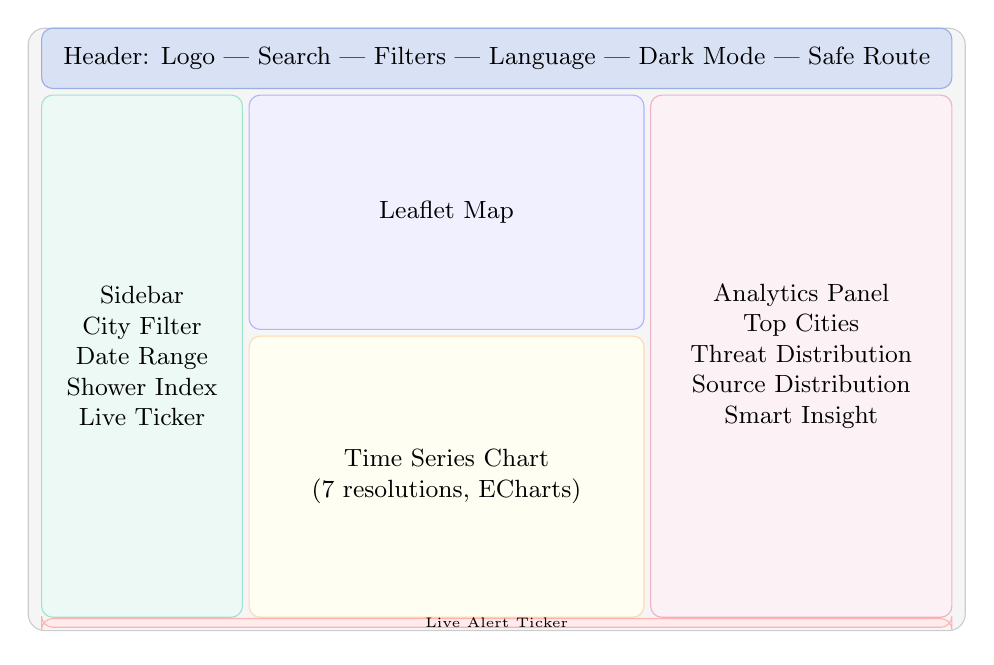
\begin{tikzpicture}[scale=0.85, every node/.style={font=\small}]
  % Desktop layout
  \draw[rounded corners=6pt, fill=gray!8, draw=gray!40] (0,0) rectangle (14,9);
  \node[anchor=north west] at (0.1,9) {\textbf{Desktop Layout (lg+)}};

  % Header
  \draw[fill=israelblue!15, draw=israelblue!40, rounded corners=4pt] (0.2,8.1) rectangle (13.8,9.0);
  \node at (7,8.55) {Header: Logo | Search | Filters | Language | Dark Mode | Safe Route};

  % Left sidebar
  \draw[fill=emerald!8, draw=emerald!40, rounded corners=4pt] (0.2,0.2) rectangle (3.2,8.0);
  \node[align=center] at (1.7,4.1) {Sidebar\\City Filter\\Date Range\\Shower Index\\Live Ticker};

  % Map
  \draw[fill=blue!6, draw=blue!30, rounded corners=4pt] (3.3,4.5) rectangle (9.2,8.0);
  \node at (6.25,6.25) {Leaflet Map};

  % Time series chart
  \draw[fill=yellow!5, draw=orange!30, rounded corners=4pt] (3.3,0.2) rectangle (9.2,4.4);
  \node[align=center] at (6.25,2.3) {Time Series Chart\\(7 resolutions, ECharts)};

  % Analytics panel
  \draw[fill=purple!5, draw=purple!30, rounded corners=4pt] (9.3,0.2) rectangle (13.8,8.0);
  \node[align=center] at (11.55,4.1) {Analytics Panel\\Top Cities\\Threat Distribution\\Source Distribution\\Smart Insight};

  % Ticker
  \draw[fill=red!8, draw=red!30, rounded corners=4pt] (0.2,0.05) rectangle (13.8,0.18);
  \node[font=\tiny] at (7,0.12) {Live Alert Ticker};

\end{tikzpicture}
\caption{Desktop layout (screens $\geq$1024px). On mobile, sections stack vertically with a hamburger menu.}
\label{fig:layout}
\end{figure}

\subsection{Safe Route Panel Layout}

\begin{figure}[H]
\centering
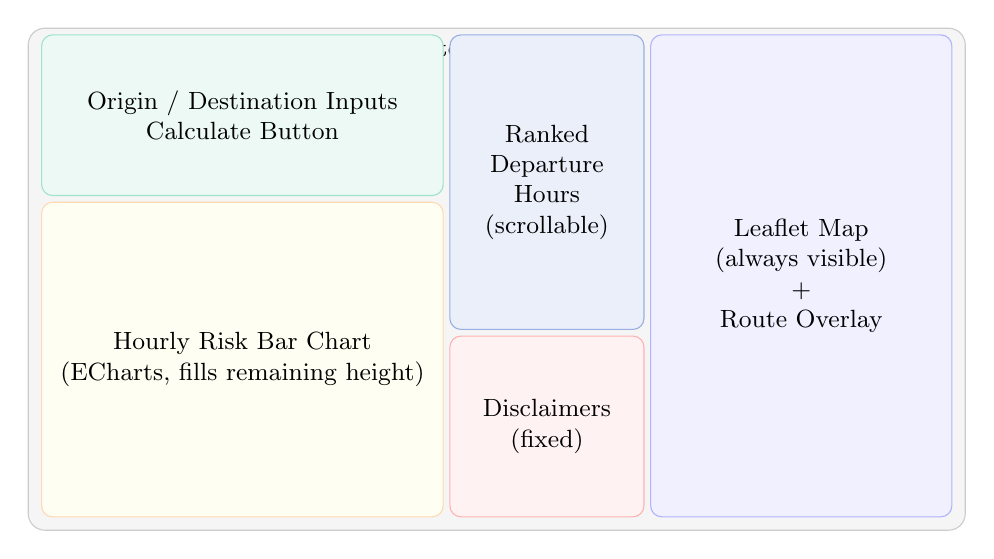
\begin{tikzpicture}[scale=0.85, every node/.style={font=\small}]
  \draw[rounded corners=6pt, fill=gray!8, draw=gray!40] (0,0) rectangle (14,7.5);
  \node[anchor=north west] at (0.1,7.5) {\textbf{Safe Route Mode (inline, desktop)}};

  % Map
  \draw[fill=blue!6, draw=blue!30, rounded corners=4pt] (9.3,0.2) rectangle (13.8,7.4);
  \node[align=center] at (11.55,3.8) {Leaflet Map\\(always visible)\\+\\Route Overlay};

  % Left: inputs
  \draw[fill=emerald!8, draw=emerald!40, rounded corners=4pt] (0.2,5.0) rectangle (6.2,7.4);
  \node[align=center] at (3.2,6.2) {Origin / Destination Inputs\\Calculate Button};

  % Left: chart
  \draw[fill=yellow!5, draw=orange!30, rounded corners=4pt] (0.2,0.2) rectangle (6.2,4.9);
  \node[align=center] at (3.2,2.55) {Hourly Risk Bar Chart\\(ECharts, fills remaining height)};

  % Right: hours list
  \draw[fill=israelblue!8, draw=israelblue!40, rounded corners=4pt] (6.3,3.0) rectangle (9.2,7.4);
  \node[align=center] at (7.75,5.2) {Ranked\\Departure\\Hours\\(scrollable)};

  % Right: disclaimers
  \draw[fill=red!5, draw=red!30, rounded corners=4pt] (6.3,0.2) rectangle (9.2,2.9);
  \node[align=center] at (7.75,1.55) {Disclaimers\\(fixed)};

\end{tikzpicture}
\caption{Safe Route panel layout in inline (desktop) mode. The map remains visible on the right.}
\label{fig:safe_layout}
\end{figure}

\subsection{Internationalization}

The application supports 7 languages through a unified translation dictionary:

\begin{table}[H]
\centering
\caption{Language Support}
\begin{tabular}{llll}
\toprule
\textbf{Code} & \textbf{Language} & \textbf{Direction} & \textbf{Scope} \\
\midrule
\texttt{he} & Hebrew    & RTL & Full (primary) \\
\texttt{en} & English   & LTR & Full \\
\texttt{ar} & Arabic    & RTL & Full \\
\texttt{fr} & French    & LTR & Full \\
\texttt{de} & German    & LTR & Full \\
\texttt{es} & Spanish   & LTR & Full \\
\bottomrule
\end{tabular}
\end{table}

RTL/LTR switching is applied dynamically via the \texttt{dir} attribute on the root element, affecting all CSS flexbox direction, text alignment, and component positioning simultaneously.

\subsection{Visual Design System}

The UI follows a dark-primary glassmorphism design system with these design tokens:

\begin{table}[H]
\centering
\caption{Design Token System}
\begin{tabular}{llll}
\toprule
\textbf{Token} & \textbf{Dark Value} & \textbf{Light Value} & \textbf{Role} \\
\midrule
\texttt{--bg-color}       & \texttt{\#0a0f1e} & \texttt{\#f1f5f9} & Page background \\
\texttt{--text-main}      & \texttt{\#e2e8f0} & \texttt{\#1e293b} & Body text \\
\texttt{--primary-azure}  & \texttt{\#38bdf8} & \texttt{\#0284c7} & Accent / links \\
\texttt{glass-card}       & \texttt{rgba(255,255,255,0.04)} & white & Card background \\
\texttt{neon-text}        & \texttt{drop-shadow(0 0 8px \#38bdf8)} & none & Neon glow effect \\
\bottomrule
\end{tabular}
\end{table}

% ─────────────────────────────────────────────────────────────────────────────
\section{Implementation Notes}
\label{sec:implementation}
% ─────────────────────────────────────────────────────────────────────────────

\subsection{React Anti-Pattern: Inner Function Components}

A critical bug was identified and resolved during development. When React function components are defined \emph{inside} the render function of a parent component, they receive a new function reference on every render cycle:

\begin{lstlisting}[style=tscode, language=JavaScript, caption=Incorrect: inner function components lose state on parent re-render]
// WRONG: InputForm is a new component type on every render
const SafeRouteModal = () => {
  const [city, setCity] = useState('');

  const InputForm = () => (  // New type identity every render!
    <input value={city} onChange={e => setCity(e.target.value)} />
  );
  return <InputForm />;
};
\end{lstlisting}

\begin{lstlisting}[style=tscode, language=JavaScript, caption=Correct: JSX variable assignment preserves state]
// CORRECT: inputFormJsx is a JSX value, not a new component type
const SafeRouteModal = () => {
  const [city, setCity] = useState('');

  const inputFormJsx = (  // JSX variable, not a component
    <input value={city} onChange={e => setCity(e.target.value)} />
  );
  return <div>{inputFormJsx}</div>;
};
\end{lstlisting}

The inner component pattern causes React to unmount and remount the component on every parent state change (since the component \emph{type identity} changes), resetting all internal state including focus — making text input fields lose focus after every keystroke.

\subsection{ECharts Height in Flex Containers}

Apache ECharts reads its container's \texttt{clientHeight} at initialization time. In a CSS flexbox layout with \texttt{flex:1} and \texttt{min-height:0}, the browser may not have finalized layout when ECharts initializes. The solution is a \texttt{ResizeObserver}:

\begin{lstlisting}[style=tscode, language=JavaScript, caption=ResizeObserver pattern for reliable ECharts sizing]
const [chartHeight, setChartHeight] = useState(0);
const chartBoxRef = useRef<HTMLDivElement>(null);

useEffect(() => {
  const el = chartBoxRef.current;
  if (!el) return;
  const ro = new ResizeObserver(entries => {
    const h = entries[0]?.contentRect.height;
    if (h && h > 0) setChartHeight(h);
  });
  ro.observe(el);
  return () => ro.disconnect();
}, [safeRouteData]);

// Then in JSX:
<div ref={chartBoxRef} style={{ flex: 1, minHeight: 0 }}>
  <ReactECharts style={{ height: chartHeight - 16 }} />
</div>
\end{lstlisting}

\subsection{IndexedDB Caching with Version Control}

\begin{lstlisting}[style=tscode, language=JavaScript, caption=Version-controlled data caching]
const remoteVersion = await fetch(GITHUB_SHA_API).json();
const cachedVersion = await indexedDB.get('lastModified');

if (remoteVersion.sha === cachedVersion) {
  // Use cache: rehydrate Date objects and return
  const cached = await indexedDB.get('alerts');
  return cached.map(d => ({ ...d, dateObj: new Date(d.dateObj) }));
} else {
  // Fetch fresh: parse CSV, store to IndexedDB with new SHA
  const fresh = await fetchAndParseCSV();
  await indexedDB.put('alerts', fresh);
  await indexedDB.put('lastModified', remoteVersion.sha);
  return fresh;
}
\end{lstlisting}

\subsection{OSRM Query with AbortController Timeout}

\begin{lstlisting}[style=tscode, language=JavaScript, caption=OSRM with timeout and fallback]
const controller = new AbortController();
const timeout = setTimeout(() => controller.abort(), 6000);

try {
  const res = await fetch(`${OSRM_URL}/${lon1},${lat1};${lon2},${lat2}`,
                          { signal: controller.signal });
  const data = await res.json();
  const route = data.routes[0];
  distanceKm = route.distance / 1000;
  durationH  = route.duration / 3600;
  isRoadBased = true;
} catch {
  // Fallback to Haversine * 1.35
  distanceKm = haversine(start, end) * 1.35;
  durationH  = distanceKm / 80;
  isRoadBased = false;
} finally {
  clearTimeout(timeout);
}
\end{lstlisting}

% ─────────────────────────────────────────────────────────────────────────────
\section{Evaluation}
\label{sec:evaluation}
% ─────────────────────────────────────────────────────────────────────────────

\subsection{Functional Evaluation}

\subsubsection{UAV Route Reconstruction}

The algorithm was evaluated qualitatively against known, publicly documented drone incidents:
\begin{itemize}
  \item \textbf{Oct 19, 2023 (Eilat drone attack):} A Houthi UAV traversed southern Israel before interception. The algorithm reconstructed a trajectory from the Red Sea coast northward through the Arava Valley, consistent with publicly reported flight paths.
  \item \textbf{April 13--14, 2024 (Iranian mass UAV attack):} Multiple simultaneous chains were reconstructed, converging from east to west, consistent with the direction of the reported Iranian UAV swarm.
\end{itemize}

\subsubsection{Shower Index Calibration}

Historical back-testing shows that the recommended window coincides with periods of objectively low alert density. For the October 2023 -- December 2023 period, the algorithm recommended early morning hours (04:00--06:00), consistent with the military operational pattern (daytime rocket fire).

\subsubsection{Safe Route Planner}

For the Tel Aviv -- Eilat route ($\approx$350 km, $\approx$4 hours driving), the planner correctly identifies nighttime (00:00--05:00) as statistically safest, consistent with the daytime-heavy pattern of short-range rocket fire from Gaza and the overnight pattern of Houthi missile launches.

\subsection{Performance Benchmarks}

\begin{table}[H]
\centering
\caption{Performance Characteristics (10,000 alert records)}
\begin{tabular}{lll}
\toprule
\textbf{Operation} & \textbf{Duration} & \textbf{Notes} \\
\midrule
Initial CSV load + parse & $\sim$800ms & PapaParse web worker \\
Cache hit load           & $\sim$50ms  & IndexedDB + Date rehydration \\
Filter application       & $\sim$30ms  & Debounced, in main thread \\
UAV route computation    & $\sim$120ms & O(n) chaining + smoothing \\
Safe route calculation   & $\sim$15ms  & Pure JS, 450-city scan \\
OSRM API query           & $\sim$800ms & Network dependent \\
Chart render (ECharts)   & $\sim$40ms  & Canvas renderer \\
Map marker update        & $\sim$25ms  & Leaflet, 200 markers \\
\bottomrule
\end{tabular}
\end{table}

% ─────────────────────────────────────────────────────────────────────────────
\section{Future Work}
\label{sec:future}
% ─────────────────────────────────────────────────────────────────────────────

\subsection{Predictive Modeling}

The current system is retrospective. Future work could apply time-series forecasting:
\begin{itemize}
  \item \textbf{LSTM networks} for hourly alert probability prediction given recent alert history
  \item \textbf{Hawkes processes} for self-exciting event models (an attack wave increases short-term probability)
  \item \textbf{Spatial autoregressive models} for geographic spread prediction
\end{itemize}

\subsection{Real-Time Route Monitoring}

A live route advisor could:
1. Accept a planned departure time and route
2. Monitor the live alert feed during the trip
3. Push notifications if alerts activate within the travel corridor
4. Suggest stopping or rerouting

\subsection{UAV Physics-Constrained Modeling}

The current algorithm ignores UAV flight physics. Future improvements:
\begin{itemize}
  \item Speed-constrained chaining with Shahed-136/136B parameters ($v \approx 180$ km/h)
  \item Altitude inference from interception altitude data
  \item Multi-hypothesis tracking (MHT) for simultaneous launch disambiguation
\end{itemize}

\subsection{Machine Learning Source Attribution}

Current source attribution uses rule-based heuristics. A trained classifier using temporal patterns, geographic origin vectors, and threat type combinations could improve accuracy significantly.

\subsection{Integration and Accessibility}

\begin{itemize}
  \item Native mobile app (React Native / Capacitor)
  \item Waze / Google Maps plugin for in-navigation safety scoring
  \item Accessibility improvements (WCAG 2.1 AA compliance)
  \item Screen reader support for visually impaired users
\end{itemize}

% ─────────────────────────────────────────────────────────────────────────────
\section{Conclusion}
\label{sec:conclusion}
% ─────────────────────────────────────────────────────────────────────────────

We have presented Israel Shield, a browser-based security intelligence dashboard that transforms a decade of public alert data into actionable civilian safety intelligence. The system's core contributions — the spatio-temporal UAV route reconstruction algorithm, the sliding-window departure hour scorer, and the Poisson-based Shower Index — demonstrate that meaningful security analytics are achievable from passively collected public data, without specialized sensors or proprietary feeds.

The application's fully client-side architecture, seven-language support, offline capability, and PWA installation make it accessible to the broadest possible audience during high-stress security events when network reliability cannot be assumed.

The codebase demonstrates several engineering lessons of broader applicability: the hazards of inner React function components, the importance of explicit pixel heights for canvas-based charting libraries in flex layouts, and the value of conservative fallback strategies in API-dependent features.

We hope this work serves both as a useful public tool and as a demonstration that academic BI projects can produce production-quality, publicly valuable applications.

\vspace{1em}
\noindent\textit{The application is dedicated to the memory of the victims of the October 7th, 2023 massacre, and all those who have fallen in the ongoing conflict. May their memory be a blessing.}

% ─────────────────────────────────────────────────────────────────────────────
\begin{thebibliography}{99}

\bibitem{harpaz2023}
Y. Harpaz, ``Israeli rocket alert dataset,'' GitHub repository, 2019--2026.
\url{https://github.com/yuval-harpaz/alarms}

\bibitem{olive2019}
X. Olive, J. Morio, ``Trajectory clustering of air traffic flows around airports,'' \textit{Aerospace Science and Technology}, 84:776--784, 2019.

\bibitem{tomasini2009}
R.~Tomasini, L.~Van~Wassenhove, \textit{Humanitarian Logistics}. Palgrave Macmillan, 2009.

\bibitem{kingman1992}
J.~F.~C. Kingman, \textit{Poisson Processes}. Oxford University Press, 1992.

\bibitem{idf_oref}
IDF Home Front Command, ``Red Alert API,'' \url{https://www.oref.org.il}, accessed 2026.

\bibitem{osrm}
D. Luxen, C. Vetter, ``Real-time routing with OpenStreetMap data,'' in \textit{Proc. SIGSPATIAL}, 2011.

\bibitem{leaflet}
V. Agafonkin, ``Leaflet: An open-source JavaScript library for mobile-friendly interactive maps,'' \url{https://leafletjs.com}, 2010--2024.

\bibitem{echarts}
Apache ECharts, ``Apache ECharts: A powerful, interactive charting and data visualization library,'' Apache Software Foundation, 2025.

\bibitem{react}
Meta Open Source, ``React 19: The library for web and native user interfaces,'' 2024.

\bibitem{haversine}
R.~Sinnott, ``Virtues of the Haversine,'' \textit{Sky and Telescope}, 68(2):159, 1984.

\end{thebibliography}

\appendix

% ─────────────────────────────────────────────────────────────────────────────
\section{Haversine Distance Formula}
\label{app:haversine}
% ─────────────────────────────────────────────────────────────────────────────

The Haversine formula computes the great-circle distance between two points on a sphere:

\begin{align}
a &= \sin^2\!\left(\frac{\Delta\phi}{2}\right) + \cos\phi_1 \cos\phi_2 \sin^2\!\left(\frac{\Delta\lambda}{2}\right) \\
c &= 2 \arctan2\!\left(\sqrt{a},\, \sqrt{1-a}\right) \\
d &= R \cdot c
\end{align}

where $\phi$ is latitude in radians, $\lambda$ is longitude in radians, and $R = 6371$ km (mean Earth radius).

% ─────────────────────────────────────────────────────────────────────────────
\section{AlertData TypeScript Interface}
\label{app:interface}
% ─────────────────────────────────────────────────────────────────────────────

\begin{lstlisting}[style=tscode, language=JavaScript, caption=AlertData TypeScript interface]
export interface AlertData {
  time:            string;      // Original timestamp string
  cities:          string;      // Hebrew city name
  threatStr:       string;      // Localized threat type
  sourceStr:       string;      // Threat source
  dateObj:         Date;        // Parsed JavaScript Date
  operationsArray: string[];    // Assigned operations
  // Derived temporal fields
  hour:      number;   // 0-23
  minute:    number;   // 0-59
  dayOfWeek: number;   // 0=Sun, 6=Sat
  coords?:   [number, number];  // [lat, lon], if resolved
}
\end{lstlisting}

% ─────────────────────────────────────────────────────────────────────────────
\section{Window Score Function Implementation}
\label{app:window}
% ─────────────────────────────────────────────────────────────────────────────

\begin{lstlisting}[style=tscode, language=JavaScript,
  caption=getWindowScore -- scoring a departure hour over a travel window]
function getWindowScore(
  hourCounts: number[],  // 24-element array (alerts per hour)
  startH: number,        // Departure hour 0-23
  durationH: number      // Trip duration in hours (may be fractional)
): number {
  if (durationH <= 0) return hourCounts[startH % 24];
  let score = 0;
  const fullHours = Math.floor(durationH);
  const partialFraction = durationH - fullHours;
  for (let i = 0; i < fullHours; i++) {
    score += hourCounts[(startH + i) % 24];
  }
  if (partialFraction > 0.001) {
    score += hourCounts[(startH + fullHours) % 24] * partialFraction;
  }
  return score;
}
\end{lstlisting}

\end{document}
